\subsection{Das Ausgangssignal}
\subsubsection{... nach dem Mischen durch den Detector}
Als erstes wird ein Signal mit einer Frequenz $f_\text{sig} = \SI{1}{\kilo\hertz}$ und einer Amplitude $U_{0,\text{sig}} = \SI{10}{\milli\volt}$ mit einer Referenz-Spannung gleicher Frequenz und der Amplitude $U_{0,\text{ref}} = \SI{30}{\volt}$ am Detector (bzw. Mischer) überlagert. Die resultierende und am Oszilloskop zu beobachtende Spannung ist in den Abbildungen \ref{Verschiebung_0} bis \ref{Verschiebung_315} dargestellt. \\
\begin{figure}[h!]
	\begin{subfigure}{0.5\textwidth}
		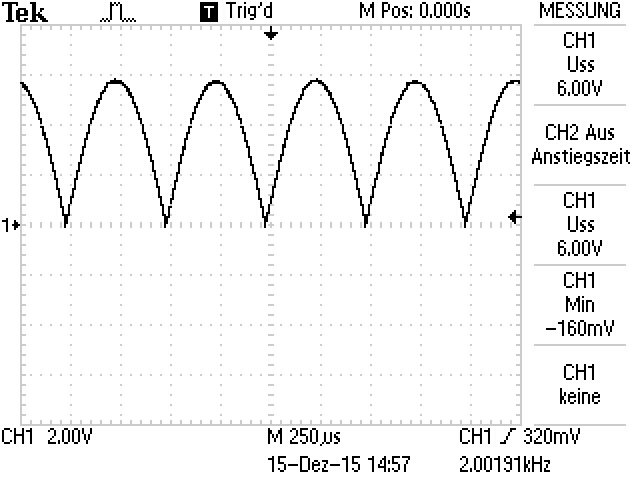
\includegraphics[width = \textwidth]{Oszilloskop-Bilder/ohne_345.JPG}
		\caption{ohne Rauschen}
	\end{subfigure}
	\begin{subfigure}{0.5\textwidth}
		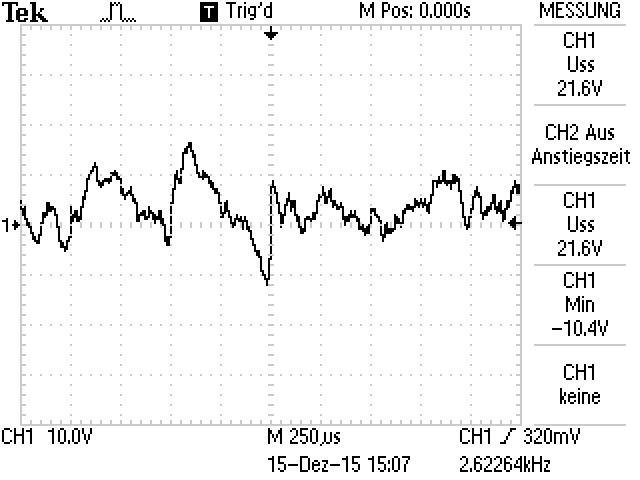
\includegraphics[width = \textwidth]{Oszilloskop-Bilder/mit_345.JPG}
		\caption{mit Rauschen}
	\end{subfigure}
	\caption{Spannungsmischung bei einer Phasendifferenz von $\Delta\phi = \SI{0}{\degree}$}
	\label{Verschiebung_0}
\end{figure}

\begin{figure}[h!]
	\begin{subfigure}{0.5\textwidth}
		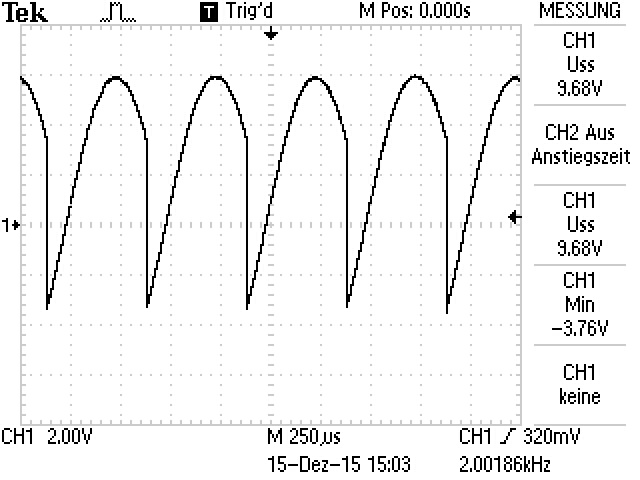
\includegraphics[width = \textwidth]{Oszilloskop-Bilder/ohne_30.JPG}
		\caption{ohne Rauschen}
	\end{subfigure}
	\begin{subfigure}{0.5\textwidth}
		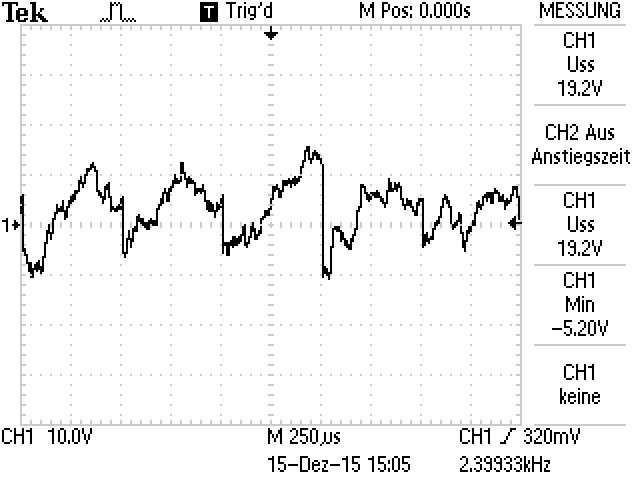
\includegraphics[width = \textwidth]{Oszilloskop-Bilder/mit_30.JPG}
		\caption{mit Rauschen}
	\end{subfigure}
\caption{Spannungsmischung bei einer Phasendifferenz von $\Delta\phi = \SI{45}{\degree}$}
\end{figure}

\begin{figure}
	\begin{subfigure}{0.5\textwidth}
		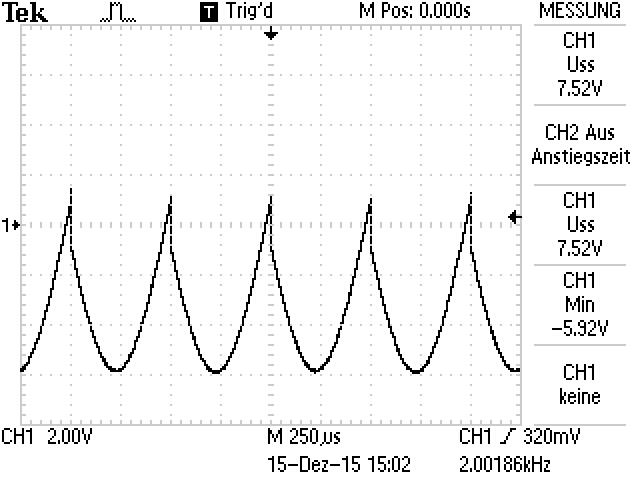
\includegraphics[width = \textwidth]{Oszilloskop-Bilder/ohne_150.JPG}
		\caption{ohne Rauschen}
	\end{subfigure}
	\begin{subfigure}{0.5\textwidth}
		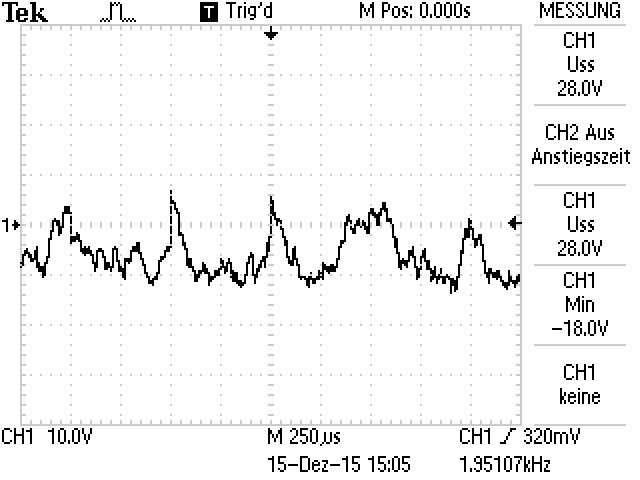
\includegraphics[width = \textwidth]{Oszilloskop-Bilder/mit_150.JPG}
		\caption{mit Rauschen}
	\end{subfigure}
\caption{Spannungsmischung bei einer Phasendifferenz von $\Delta\phi = \SI{165}{\degree}$}
\end{figure}

\begin{figure}
	\begin{subfigure}{0.5\textwidth}
		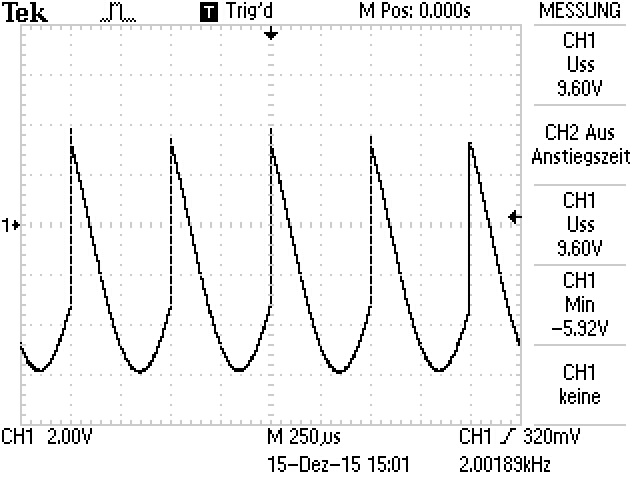
\includegraphics[width = \textwidth]{Oszilloskop-Bilder/ohne_210.JPG}
		\caption{ohne Rauschen}
	\end{subfigure}
	\begin{subfigure}{0.5\textwidth}
		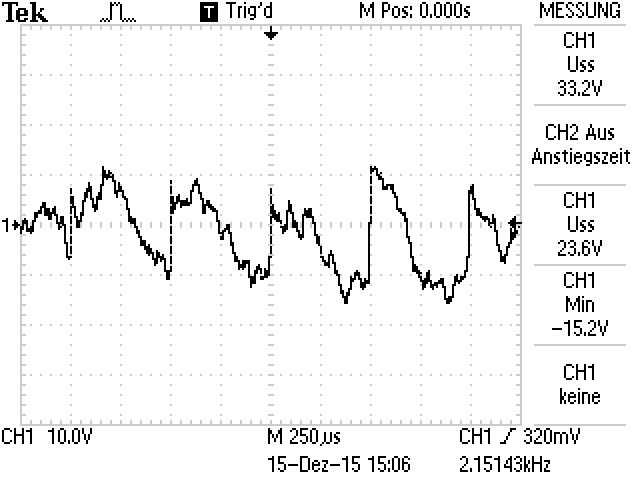
\includegraphics[width = \textwidth]{Oszilloskop-Bilder/mit_210.JPG}
		\caption{mit Rauschen}
	\end{subfigure}
\caption{Spannungsmischung bei einer Phasendifferenz von $\Delta\phi = \SI{225}{\degree}$}
\end{figure}

\begin{figure}
	\begin{subfigure}{0.5\textwidth}
		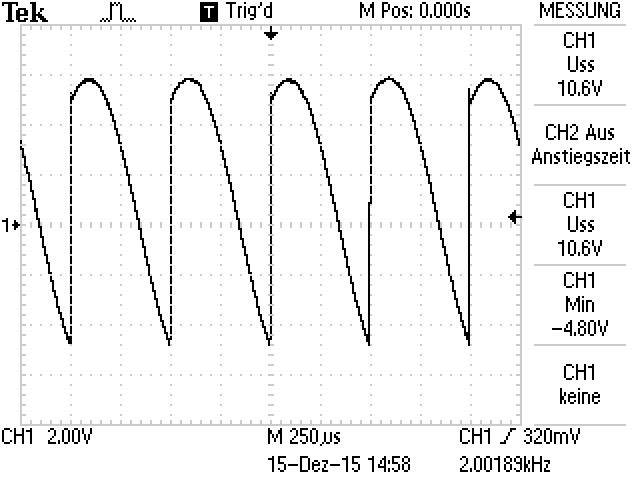
\includegraphics[width = \textwidth]{Oszilloskop-Bilder/ohne_300.JPG}
		\caption{ohne Rauschen}
	\end{subfigure}
	\begin{subfigure}{0.5\textwidth}
		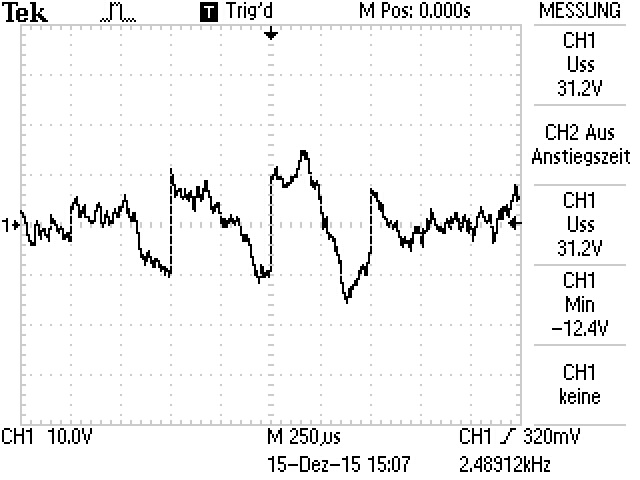
\includegraphics[width = \textwidth]{Oszilloskop-Bilder/mit_300.JPG}
		\caption{mit Rauschen}
	\end{subfigure}
\caption{Spannungsmischung bei einer Phasendifferenz von $\Delta\phi = \SI{315}{\degree}$}
\label{Verschiebung_315}
\end{figure}
\clearpage

\subsubsection{... nach dem Integrieren am Tiefpass}
In einem Lock-In-Verstärker wird die im vorigen Abschnitt beschriebene \glqq Misch-Spannung\grqq\ noch über einen Tiefpass integriert. Als Zeitperiode wird dafür $T = \SI{1}{\second}$ gewählt. Der Wert dieses Integrals wird für verschiedene Phasenverschiebungen abgelesen und ist in Tabelle \ref{Integral_ohne} bzw. \ref{Integral_mit} eingetragen. \\
\ \\
\ \\
\ \\
\textbf{Das Signal ohne Rauschen} \\
Es wird im Folgenden zunächst das Signal ohne Rauschen betrachtet. Der Off-Set wird abgezogen und die Winkel zum Bogenmaß überführt. Dann kann die Funktion
\[f(\phi) = A\cos(w\phi+\phi_0)\]
auf die Messwerte gefittet werden. Mit Hilfe von Python ergeben sich so die Parameter
\begin{align}
	A_\text{ohne} &= \SI{2.04(011)}{\milli\volt} \\
	w_\text{ohne} &= \SI{1.00(004)}{} \\
	\phi_{0,\text{ohne}} &= \SI{-0.008(53)}{\pi}
\end{align}
Die dadurch beschriebene Kurve ist in Abbildung \ref{Fit_ohne} zusammen mit den Messwerten und der theoretisch mit \eqref{Ausgangssignal} zu erwartenden Kurve dargestellt. \\
\begin{table}[h!]
\begin{center}
\begin{tabular}{c | c | c}
	Phasenverschiebung in \si{\degree} & Integral in \si{\volt} & Off-Set in \si{\degree} \\
	\hline
	0   & -9.5 & +165 \\
	15  & 6.2 & -15 \\
	90  & 1.5 & +165 \\
	150 & -6.9 & -15 \\
	180 & 9.1 & +165 \\
	210 & -5.7 & -15 \\
	255 & 0 & -15 \\
	270 & -1.5 & +165 \\
	315 & -7.6 & +165 \\
	345 & 7 & -15
\end{tabular}
\caption{Integral (bzw. Gleichspannung) nach dem Tiefpass für verschiedene Phasenverschiebungen bei einem \glqq reinen\grqq\ Signal}
\label{Integral_ohne}
\end{center}
\end{table}
\begin{figure}[h!]
	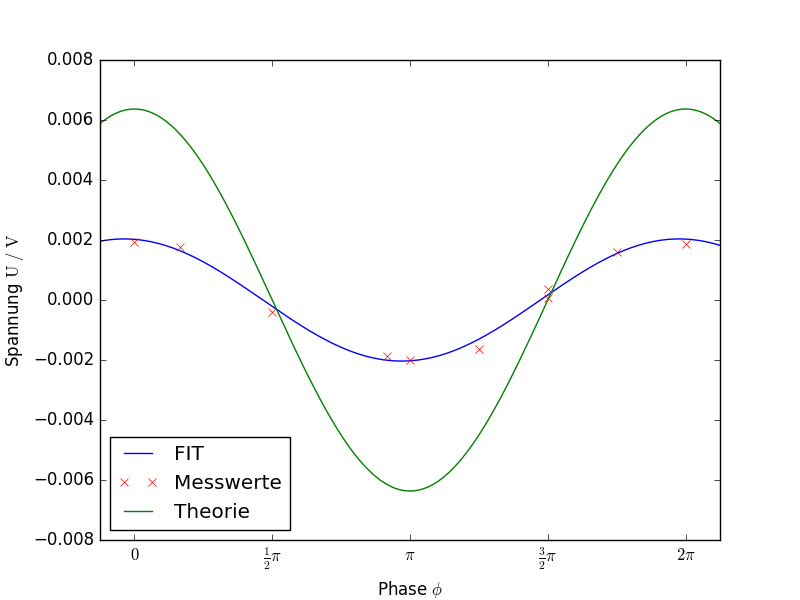
\includegraphics[width = \textwidth]{Phase_mit.png}
	\caption{Messwerte, gefittete Kurve und theoretisch erwartete Kurve bei einer Spannung ohne Rauschen}
	\label{Fit_ohne}
\end{figure} \\
\ \\
\ \\
\ \\
\ \\
\ \\
\textbf{Das Signal mit Rauschen} \\
Dieser Fit wird nun auch mit den Werten des verrauschten Signals gemacht. Die Parameter hierbei sind
\begin{align}
	A_\text{mit} &= \SI{2.036(0085)}{\milli\volt} \\
	w_\text{mit} &= \SI{0.993(0029)}{} \\
	\phi_{0,\text{mit}} &= \SI{0.036(0036)}{\pi}
\end{align}
\begin{table}[h!]
	\begin{center}
		\begin{tabular}{c | c | c}
			Phasenverschiebung in \si{\degree} & Integral in \si{\volt} & Off-Set in \si{\degree} \\
			 & bei einem Gain von 4000 & \\
			\hline
			0   & 7.8 & +0 \\
			15  & 7.1 & -15 \\
			90  & -1.6 & +0 \\
			150 & -7.5 & -15 \\
			180 & -8.0 & +0 \\
			210 & -6.5 & -15 \\
			255 & 0.3 & -15 \\
			270 & 1.5 & +0 \\
			315 & 6.4 & +0 \\
			345 & 7.5 & -15
		\end{tabular}
		\caption{Integral (bzw. Gleichspannung) nach dem Tiefpass für verschiedene Phasenverschiebungen bei einem verrauschten Signal}
		\label{Integral_mit}
	\end{center}
\end{table} \\
Auch dieser Fit wird zusammen mit der zu erwartenden Kurve und den Messwerten geplottet (Abbildung \ref{Fit_mit}).
\begin{figure}[h!]
	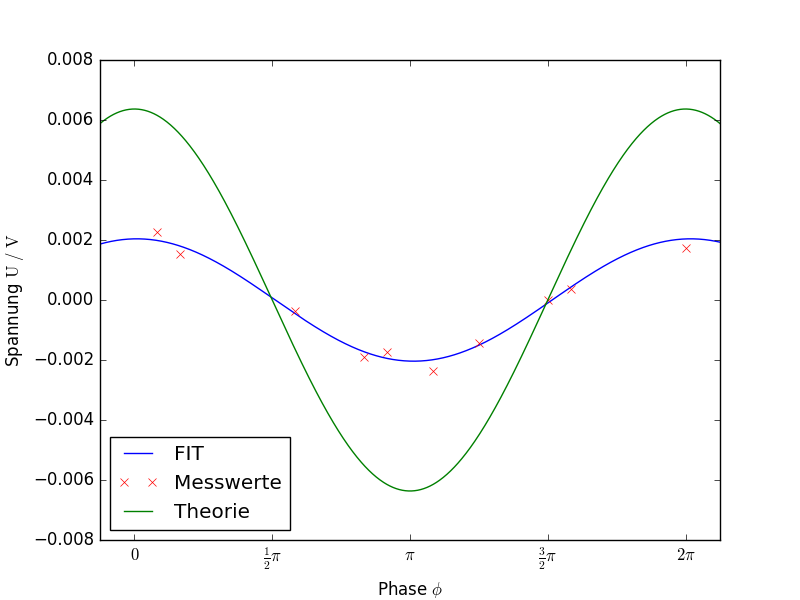
\includegraphics[width = \textwidth]{Phase_ohne.png}
	\caption{Messwerte, gefittete Kurve und theoretisch erwartete Kurve bei einer Spannung mit Rauschen}
	\label{Fit_mit}
\end{figure}
\clearpage
\subsection{Die Rauschunterdrückung}
Beim Versuchsaufbau mit der LED wird bei verschiedenen Abständen die Ausgangsspannung nach dem Tiefpass aufgenommen. Nach Abzug der Verstärkungs-Multiplikatoren (Gains) ergeben sich die Werte aus Tabelle \ref{Tabelle_Lampe}.
\begin{table}[b!]
\begin{center}
\begin{tabular}{c | c}
	Abstand $r$ zur Lampe in \si{\metre} & Integral (bzw. Spannung) $U$ in \si{\milli\volt} \\
	\hline
	0.17 & 17.25 \\
	0.27 & 3.500 \\
	0.37 & 1.250 \\
	0.47 & 0.600 \\
	0.57 & 0.350 \\
	0.67 & 0.250 \\
	0.77 & 0.180 \\
	0.87 & 0.130 \\
	0.97 & 0.103 \\
	1.07 & 0.080 \\
	1.17 & 0.063 \\
	1.27 & 0.055 \\
	1.37 & 0.047 \\
	1.47 & 0.042 \\
	1.57 & 0.038 \\
	1.67 & 0.032 \\
	1.77 & 0.028 \\
	1.87 & 0.025 \\
	1.97 & 0.022
\end{tabular}
\caption{Abstand zur LED und registrierte Spannung}
\label{Tabelle_Lampe}
\end{center}
\end{table}
Durch eine Regression der Form
\begin{equation}\label{Regression_Gleichung}
	\ln U = \alpha\ln r +\beta
\end{equation}
lässt sich der lineare Zusammenhang zwischen $\ln r$ und $\ln U$ (siehe Abbildung \ref{Regression}) erkennen.
\begin{figure}[h!]
	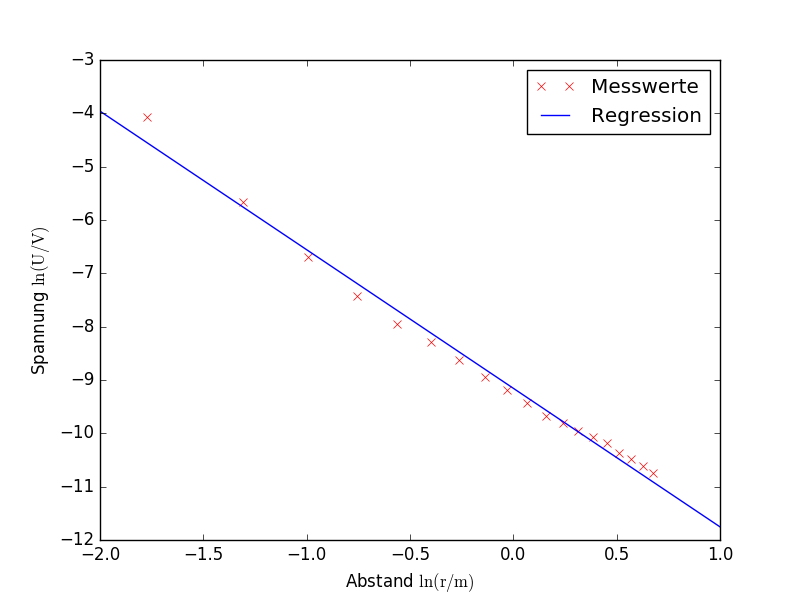
\includegraphics[width = 0.95\textwidth]{Regression.png}
	\caption{Regressionsgerade}
	\label{Regression}
\end{figure}
Die mit Python errechneten Parameter sind
\begin{align}
	\alpha &= \SI{-2.598(0065)}{\ln\left(\volt\per\metre\right)} \\
	\beta &= \SI{-9.155(0045)}{\ln\volt}\ .
\end{align}
Durch Umstellen von Gleichung \eqref{Regression_Gleichung} ergibt sich die Funktion
\begin{equation}
	U(r) = \exp(\beta) r^\alpha\ ,
\end{equation}
welche in Abbildung \ref{U(r)} zu sehen ist.
\begin{figure}[h!]
	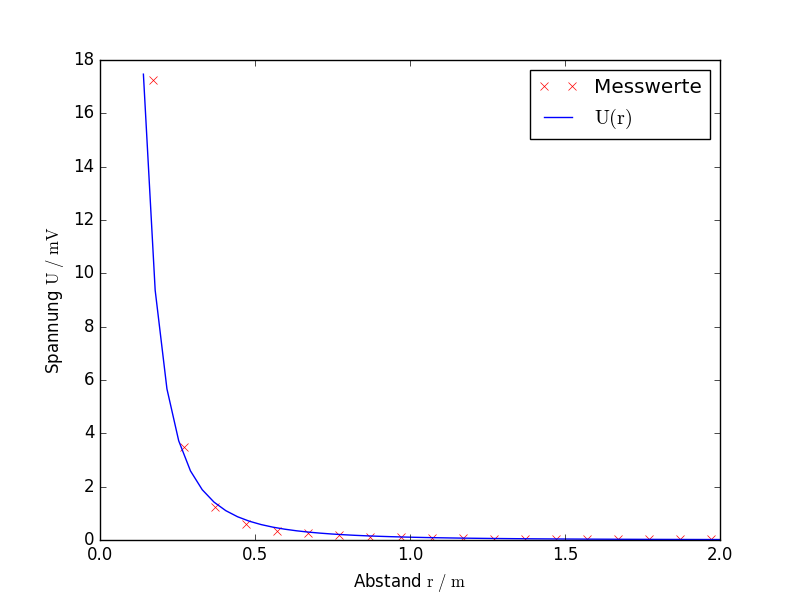
\includegraphics[width = 0.95\textwidth]{U(r).png}
	\caption{Zusammenhang zwischen $U$ und $r$}
	\label{U(r)}
\end{figure}